\section{Higgs Physics}
\paragraph{a)}
First let
\begin{equation}
	V(\eta) = \mu^2 \abs{\eta(\mathbf{r}, t)}^2 + \lambda \abs{\eta(\mathbf{r}, t)}^4
\end{equation}
and the perform the transformation
\begin{equation}
	\eta(\mathbf{r}, t) \to \eta(\mathbf{r}, t) e^{i\beta} \label{eq:transformation}
\end{equation}
now the first equation becomes
\begin{align}
	V(\eta) &= \mu^2 \abs{\eta(\mathbf{r}, t) e^{i\beta}}^2 + \lambda \abs{\eta(\mathbf{r}, t) e^{i\beta}}^4 = \mu^2 \abs{\eta(\mathbf{r}, t)}^2 \times \abs{e^{i\beta}}^2 + \lambda \abs{\eta(\mathbf{r}, t)}^4 \times \abs{e^{i\beta}}^4\\
	&= \mu^2 \abs{\eta(\mathbf{r}, t)}^2 \times 1^2 + \lambda \abs{\eta(\mathbf{r}, t)}^4 \times 1^4 = \mu^2 \abs{\eta(\mathbf{r}, t)}^2 + \lambda \abs{\eta(\mathbf{r}, t)}^4.
\end{align}
We get the exact same as before the transformation. Thus it is $V(\eta)$ is invariant under the transformation Eq. \eqref{eq:transformation}.

\paragraph{b)} Firstly an electric field separates the electron from a hydrogen atom and thus creating free protons. Then along the accelerator an electric field oscillates from positive to negative which accelerates the particle forward. By controlling the frequency the particles come as bunches instead of a continuous stream.

\paragraph{c)}
\begin{figure}[H]
	\centering
	\begin{subfigure}{0.49\textwidth}
		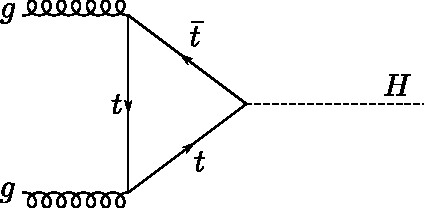
\includegraphics[width=\textwidth]{figures/gg_higgs.pdf}
		\caption{$g g \to H$}
	\end{subfigure}
	\hfill
	\begin{subfigure}{0.49\textwidth}
		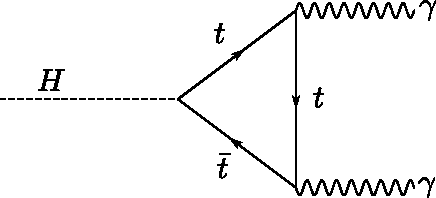
\includegraphics[width=\textwidth]{figures/Higgs_yy.pdf}
		\caption{$H \to \gamma \gamma$}
	\end{subfigure}
	\caption{Feynman diagrams for Higgs production and Higgs decay resulting in two gammas.}
\end{figure}
\paragraph{d)}

\begin{figure}
	\centering
	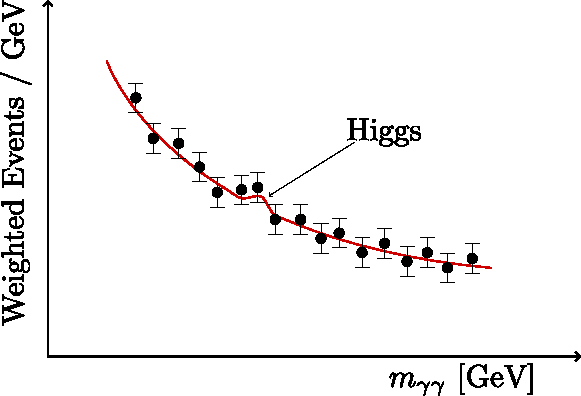
\includegraphics[width=0.8\textwidth]{figures/Higgs_detection.pdf}
	\caption{Higgs detection by gamma.}
\end{figure}


